

\begin{figure*}[t]
   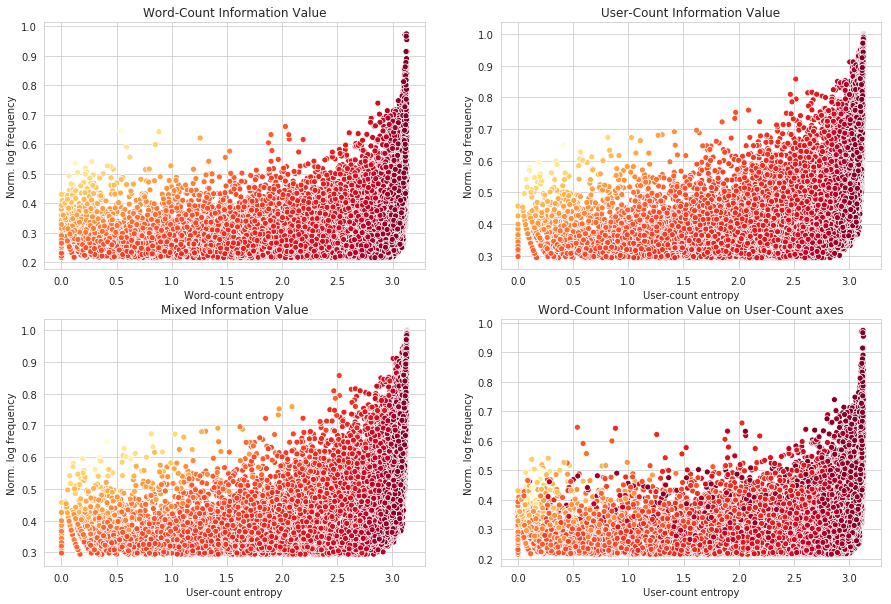
\includegraphics[width=\textwidth]{./images/entropy_log_rank.png}
   \label{fig:ivalue}
   \caption{Scatter plot of words. Horizontal axis represents user-count entropy, vertical axis represents the normalized log user-frequency of the word, and colour indicates User-count Information Value: lighter means higher value}
\end{figure*}



Figure \ref{fig:ivalue} displays the log-frequency and Entropy of words, along with the value of the respective metric. As we can see (both in the User-Count and Word-Count plots) the words we rank high in our lists are those closer to the upper-left of the plot — that is, highly-concentrated and occurring a consideriable number of times. Mixed Information Value seems to respect the User-Count order, and the last plot shows that although User-Count and Word-Count ranks are similar, they are not exactly the same as shown by the ``darker'' points close to the upper-left corner.

\todo{Agregar un listado de las 10 primeras palabras de cada listado?}

Regarding the lexicographic validation, Table \ref{tab:metric_results} display the percentage of words marked as being lexicographically interesting. The number of users of a word alone seems to be the most informative feature. 

\begin{table}[t]
\centering
\begin{tabular}{lr}
Metric                      &  \% of interesting words  \\ % &           STD \\
\hline
Word-Count       &  21.9\%   \\
User-Count       &  30.2\%  \\
Mixed            &  25.3\%  \\ %&  1.947665e+01 \\
\hline
\end{tabular}
\caption{Results of the metrics. The percentage of detected regionalisms in the first 1000 words is given for each metric: Word Information Value, User Information Value, and Mixed Information Value  }
\label{tab:metric_results}
\end{table}


